% Ported verbatim (prose unchanged) from docs/SECTION_6_DRAFT.md.
\section{Analysis}
\label{sec:analysis}

A null result earns its place in the literature only if it explains itself: which alternative explanations it has excluded, what the tested mechanisms demonstrably did learn, and what evidence would overturn the conclusion. This section takes each in turn.

\subsection{The Dissociation: Relational Memory Learns Dynamics the Emotion Readout Cannot Use}
\label{sec:dissociation}

The most informative single observation in our results is a dissociation. Across both corpora, enabling the relational-memory component \textit{improves} performance on the auxiliary shift-detection task (predicting whether a speaker's emotion has changed relative to their own previous utterance) while degrading performance on the primary emotion-classification task (shift-F1 delta, full stack minus the stack without relational memory: MELD $\mathbf{+0.0297}$: $0.6682$ vs.\ $0.6384$; IEMOCAP $\mathbf{+0.0782}$: $0.4147$ vs.\ $0.3365$, both means of $3$ seeds). The component is not failing to learn; it is learning something real about conversational dynamics that does not convert into better emotion labels once the foundation is fine-tuned. This single fact excludes the two laziest readings of our nulls. It excludes ``the relational pathway is broken or under-trained'': a broken pathway does not improve any task. And it excludes ``conversations contain no pair-level dynamical structure'': the shift head finds exactly such structure through the relational states. What remains is the reading the boundary claim proposes: the emotion-relevant portion of conversational context is already captured by a task-adapted encoder, and what the graph pathway adds beyond it is dynamics information that is genuine but redundant (or worse, distracting) for the classification readout. The premise of the shift objective is confirmed cleanly on MELD (neutral shift rate $0.39$--$0.43$ across splits versus fear/disgust/surprise at $1.5$--$2.1\times$ higher, no exception across train/dev/test) but only \textbf{partially} on IEMOCAP, where minority/less-common classes do not uniformly show elevated shift rates relative to neutral: only \texttt{angry} does so cleanly across all three splits, \texttt{happy} and \texttt{frustrated} each have one exception (both in the validation split), and \texttt{sad}/\texttt{excited} run the opposite direction. We report this plainly rather than smoothing it into a uniform premise: the auxiliary task was aimed at real structure on MELD and at weaker, more corpus-specific structure on IEMOCAP, yet the shift-F1 gain from relational memory is if anything \textit{larger} on IEMOCAP: the mechanism appears to find dynamical signal beyond what the simple minority-class/shift-rate correlation alone would predict. Either way, on MELD specifically, the structure was demonstrably not the classification bottleneck.

\begin{figure*}[t]
\centering
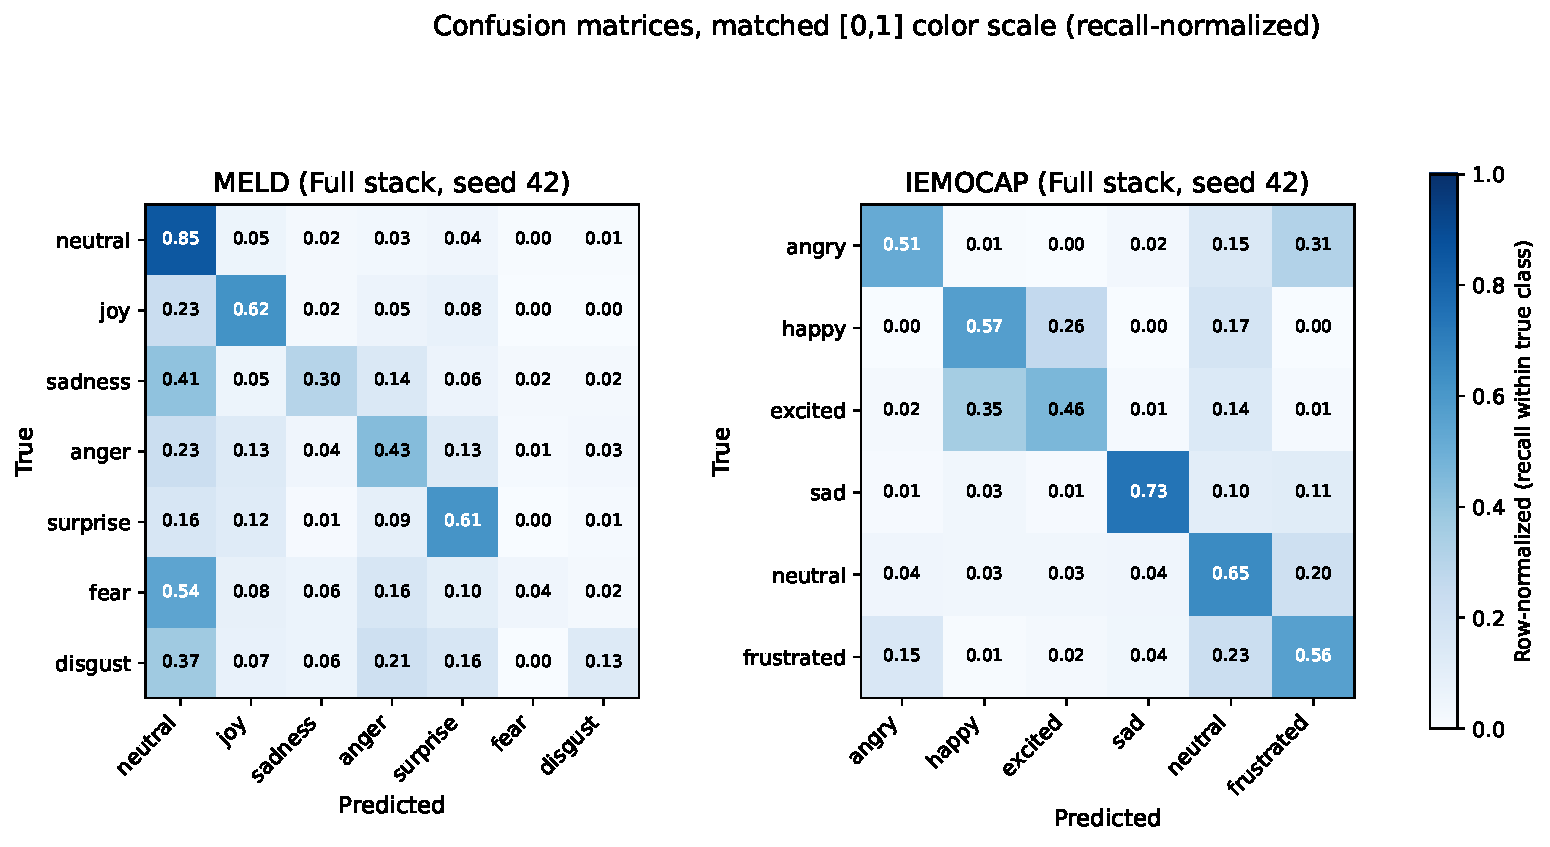
\includegraphics[width=\textwidth]{figures/confusion_matrices.pdf}
\caption{Test-set confusion matrices, row-normalized so each cell shows recall within the true class, matched $[0,1]$ color scale for direct visual comparison across corpora. Full stack configuration, seed $42$: MELD (left, seven classes) and IEMOCAP (right, six classes).}
\label{fig:confusion}
\end{figure*}

\subsection{The Edge-State Trajectories: Two Readings, Honestly Held}

The qualitative trajectories of Figure~\ref{fig:edge-norm} show a consistent signature across the sampled IEMOCAP dialogues: the relational state's norm rises rapidly at first (turn-to-turn increments above $0.1$ in every dialogue for the first four to five turns), with the steep phase tapering by turn $5$--$7$ in two of the three dialogues and continuing at a slower positive rate to roughly turn $12$ in the third, then settles into a comparatively stable regime with a roughly twofold-to-sevenfold drop in variance ($1.8\times$--$7.4\times$ across the three dialogues, front-half versus back-half standard deviation). Two interpretations fit this shape and we decline to choose between them by assertion. The first is relationship tracking: the memory acquires a representation of the dyad early and thereafter maintains it, updating conservatively, consistent with the shift-detection gains of Section~\ref{sec:dissociation}, which require the states to carry interaction-specific information. The second is generic recurrent saturation: gated recurrent cells commonly exhibit early norm growth followed by a stable operating point regardless of what they encode, and norm dynamics alone cannot distinguish content from habit. The evidence adjudicates only partially: saturation-without-content predicts no downstream utility, and the shift-task improvement shows the states are read out to some effect, so the purely vacuous reading is disfavored; but the trajectories themselves should be understood as illustrative of the mechanism's operation, not as evidence for its value: the quantitative tables carry that burden, and they carry it in the negative direction.

\subsection{What Would Falsify the Boundary Claim}

We state the claim's exposure plainly. The boundary claim would be falsified by a demonstration, under an attribution instrument at least as conservative as ours, of a consistent positive contribution from conversation-graph machinery on top of a competitively fine-tuned encoder. Three settings strike us as the most promising places to look, in descending order of our credence. First, corpora with genuinely long-horizon social structure exceeding any feasible context window (multi-session interactions, longitudinal counseling or support dialogues, communities with persistent relationships), where the relevant history is measured in thousands of turns; neither MELD's nine-utterance scenes nor IEMOCAP's single sessions test this regime, and our negative results do not extend to it. Second, tasks whose labels are themselves relational (rapport, conflict escalation, dominance) rather than per-utterance emotion, for which Section~\ref{sec:dissociation} suggests the relational states already carry usable signal. Third, foundations weaker by necessity (low-resource languages, privacy-constrained on-device encoders, domains where fine-tuning data cannot be obtained), where our own frozen-regime result ($+0.036$) predicts graph machinery still pays; the boundary claim is a claim about what happens when fine-tuning is available, not a universal deprecation. Conversely, results that would \textit{not} move us: gains reported over frozen or lightly tuned baselines (Section~\ref{sec:meld-frozen} reproduces these ourselves), gains under scratch-retrained ablations without attribution controls (Section~\ref{sec:meld-mechanism} quantifies how such designs mismeasure), and gains on split conventions or label subsets tuned after the fact.

\subsection{Threats to Validity}

Seeds and power: our claims rest on three to seven seeds; we report paired per-seed differences and standard deviations and abstain from significance tests, but effects smaller than roughly one standard deviation ($0.007$--$0.028$ depending on the comparison; narrowest for the seven-seed MELD $k{=}8$ endpoint, widest for the three-seed IEMOCAP relational-isolation estimate) are beneath our resolution, and the IEMOCAP relational estimate in particular ($-0.033 \pm 0.028$) is directionally clear but imprecise. Foundation generality: all fine-tuned foundations are RoBERTa-base with LoRA; larger encoders, full fine-tuning, or instruction-tuned models~\cite{zhang2025dialoguellm} could in principle shift the boundary in either direction, though the mechanism argument of Section~\ref{sec:dissociation} suggests the direction would be toward stronger subsumption, not weaker. Modality ceilings: acoustic and visual features are frozen throughout (probe ceilings $0.411$ and $0.335$ on MELD); a fine-tuned acoustic encoder might raise the non-textual contribution for any architecture, graph or otherwise: our claim concerns the graph machinery's marginal value, not the modalities'. Attribution instrument: zero-initialization is a soft prior toward the foundation (Section~\ref{sec:residual-construction}); we bound this concern with the frozen-regime positive control, but a component whose value requires reorganizing the shared pathway could be under-credited. Corpus scope: two English-language acted/scripted corpora; spontaneous, non-English, and text-free interaction may distribute context differently across modalities and history. Finally, literature comparisons in this paper cite published numbers and are not independently reproduced; in particular, the original implementation of our own prior system was lost to an infrastructure failure (documented in the repository), and our early re-implementation attempts are not faithful reproductions. The complete decision history, including failed designs and the incidents that shaped the methodology, is public in the project repository, and we regard that history as part of the paper's evidence.
